

\chapter{Design Concept} \label{chapter:desgin}

\section{Video Gallery}
The video Gallery in our mobile-application gives the user the possibility to watch test reviews and commercial videos of the tracked car.
\\

   
For implementing the YouTube car video gallery we used \textbf{jquery} and the jquery plug-in \textbf{jquery.youtubevideogallery}. The Design and CSS files were taken from Jack Moore's plug-ins. \cite{jqueryVideo}. His great work makes it possible to dynamically scale the size and position of the video-boxes so that they perfectly fit on every device screen! 
\\

As we can se in the figure on the next page the position and size automatically adjust to the 3 different screen sizes.    

\begin{figure}[htbp]
\centering
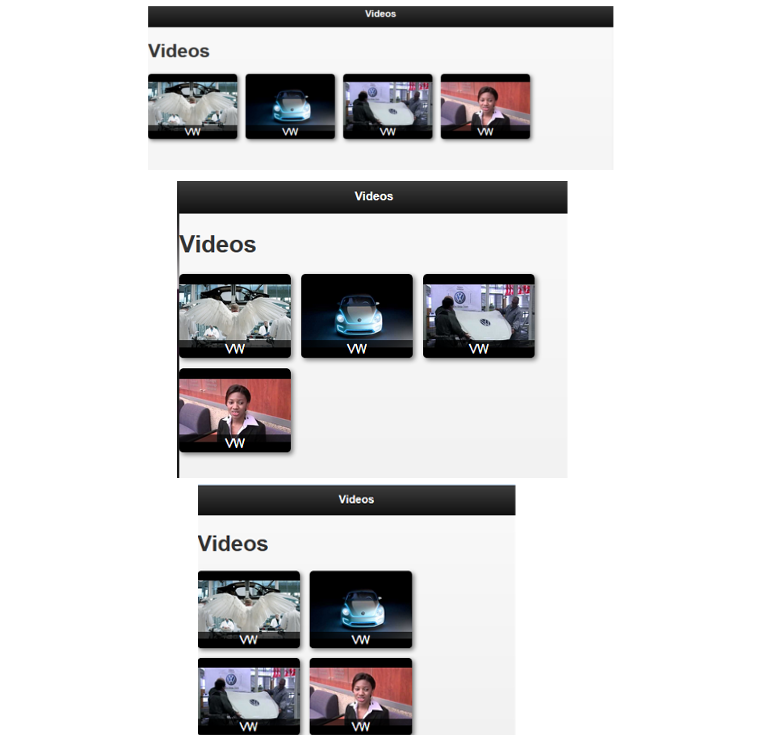
\includegraphics[width=\textwidth,height=\textheight,keepaspectratio]{graphics/dynamic.png}
\caption{dynamically fit to device screen}
\end{figure}  

\newpage
\subsection{Implementation}
We wrote a JavaScript script that appends an array of different YoutTube video url to an \textbf{ul} tag which uses the \textbf{youtube-videogallery} class.   

\begin{lstlisting}[language=html, caption= 
extracts from the video gallery src]
<ul id="Gallery" class="youtube-videogallery">
	<script>
	... 
	//append video urls
	for (var i=0; i<videos.length; i++){
		$("#Gallery").append(videos[i]);
	}
	</script>
</ul>
<!-- Use jack Mores .js and css filess to make the gallery -->
<script>
    $(document).ready(function(){
        $("ul.youtube-videogallery").youtubeVideoGallery( {plugin:'colorbox',assetFolder:'../'} );
    });
</script> 
\end{lstlisting}




\section{hallo}
my name is NASDAQ property  